\documentclass[preprint,twoside,11pt]{article}

\usepackage{blindtext}


% Any additional packages needed should be included after jmlr2e.
% Note that jmlr2e.sty includes epsfig, amssymb, natbib and graphicx,
% and defines many common macros, such as 'proof' and 'example'.
%
% It also sets the bibliographystyle to plainnat; for more information on
% natbib citation styles, see the natbib documentation, a copy of which
% is archived at http://www.jmlr.org/format/natbib.pdf

% Available options for package jmlr2e are:
%
%   - abbrvbib : use abbrvnat for the bibliography style
%   - nohyperref : do not load the hyperref package
%   - preprint : remove JMLR specific information from the template,
%         useful for example for posting to preprint servers.
%
% Example of using the package with custom options:
%
% \usepackage[abbrvbib, preprint]{jmlr2e}

\usepackage{jmlr2e}
\usepackage{tikz}
\usetikzlibrary{positioning}
\usepackage{amssymb}
\usepackage{amsmath}
\usepackage{tcolorbox}
\usepackage{mathtools}
\usepackage{enumerate}
\usepackage{algorithm}
\usepackage{algorithmicx}
\usepackage{algpseudocode}
\usepackage{pgfplots}
\pgfplotsset{compat=1.18}
\usepackage[thinc]{esdiff}
\usepackage{multirow}
\usepackage{array}
\usepackage{tabularx}
\usepackage{booktabs}

% Definitions of handy macros can go here

\newcommand{\dataset}{{\cal D}}
\newcommand{\fracpartial}[2]{\frac{\partial #1}{\partial  #2}}

% Heading arguments are {volume}{year}{pages}{date submitted}{date published}{paper id}{author-full-names}

\usepackage{lastpage}
\jmlrheading{23}{2022}{1}{1/21}{9/22}{21-0000}{Author One and Author Two}

% Short headings should be running head and authors last names

\begin{document}

\title{P2P-LLM: Collaborative LLM Inference}

\author{\name Andrew Boessen \email boessena@bc.edu \\
}

\maketitle

\begin{abstract}%   <- trailing '%' for backward compatibility of .sty file
	This project explores a framework that enables distributed running of large language models across personal computing devices connected in a peer-to-peer network.
	While current advanced AI models require substantial computing resources typically available only to large organizations,
	P2P-LLM offers an alternative approach by dividing these models into smaller parts that can be processed across multiple personal computers.
	The system includes efficient routing mechanisms to find optimal paths through the network, balancing computational speed and cost.
	To encourage participation, the project develops a fair pricing system where participants are rewarded for contributing their computing power.
	This marketplace is secured by blockchain technology, which handles payments and ensures that agreements between participants are honored.
	The P2P-LLM approach demonstrates how collaborative computing could make advanced AI more accessible while enhancing privacy and user autonomy,
	potentially transforming how these technologies are accessed in the future.
\end{abstract}

\section{Introduction}

In recent years, large language models (LLMs) have demonstrated remarkable capabilities across diverse tasks,
exhibiting unprecedented rates of improvement within a relatively brief developmental timeline.
This extraordinary progress can be primarily attributed to the immense computational resources allocated to training these models on datasets comprising
trillions of tokens, resulting in systems that subsequently demand substantial computing power for deployment.
The computational intensity of these models has resulted in significant investment,
with billions of dollars directed toward the construction of specialized super-clusters housing hundreds of thousands of GPUs dedicated to the training and serving of LLMs.
Given the substantial memory and computational requirements of state-of-the-art LLMs, most personal computing devices lack the necessary specifications to run or train these models independently.
Consequently, access to LLM capabilities is predominantly channeled through services offered by large technology corporations, which may present concerns regarding privacy, autonomy, and accessibility.

Crowdsourcing methodologies offer a promising alternative to address these limitations.
The crowdsourcing approach has demonstrated considerable success across various domains, including knowledge aggregation (Wikipedia),
real-time traffic information collection (Waze), and venture capital formation (Kickstarter).
These same foundational principles can be effectively applied to computational resource allocation and utilization.

My work explores fully decentralized crowd computing architectures,
where users establish a peer-to-peer network in which each participant can leverage the collective computational resources for individual tasks.
This structure shares conceptual similarities with BitTorrent file-sharing networks.
While current state-of-the-art language models exceed the capacity of individual personal computers,
the aggregation of distributed computational resources through a decentralized network could potentially enable users to host their own LLMs,
thereby democratizing access to advanced artificial intelligence capabilities.
\section{Realted Work}

\subsection{Crowd Computing}

The idea of pooling compute power from many computers to form a distributed supercomputer is not new. This concept of Crowd Computing
has been used ever since large networks of computer were formed. The predominant use of this method is to facilitate academic research.
Researchers publish problem that that are working on, and anyone can help contribute by volunteering to donate computing power.
Projects that have successfully used crowd computing include SETI@Home \citep{10.1145/581571.581573} and Einstein@Home \citep{Steltner_2021}.
This approach has proven to be successful in the past, but it has become less popular as the computational power of computers increased and access to supercomputers increased.
However, the use of idle compute power still has untapped applications, and the principles from crowd computing can be applied to modern tasks like LLM inference.

\subsection{P2P Networks}

LLM inference is a perfect candidate for P2P network because it has technical requirements that prohibit most personal computers from being able to run
large models with billions of parameters, and it can easily be split into small chunks that can be run on several computers at the same time. BitWorker \citep{Durand_Gasparyan_Rouvinez_Aad_Braun_Trinh_2015} is a protocol designed to compute any parallel computing task across a peer-to-peer network.
Although it is possible to apply LLM inference to this protocol, BitWorker is designed for general tasks and would not able to efficiently scale to the demands of many users.
The most notable research being done in this area is Petals \citep{borzunov2023petalscollaborativeinferencefinetuning} which is a BitTorrent like peer-to-peer network for LLM inference and finetuning.
Petals creates a network with client and servers. Clients send requests that will be processed by the servers on the network. The model is split into multiple sequential blocks of layers, and each server
in the network is capable of serving one or multiple of these blocks. In order to run an inference step, a client will find a optimal path of servers
in the network that forms the complete model and minimizes time required. In my work I explore a similar approach with a network of distributed computers that serve a specific part of the whole LLM,
but I expand upon this and add incentive mechanisms that reward nodes for donating their computational power. This incentive mechanism also facilitates optimal allocation of nodes to maximize throughput, by each
node maximizing expected revenue individually.

\section{Peer-to-Peer Network}

Fundamentally, a peer-to-peer network is a decentralized system where each devices acts as a client and a sever.
Each devices can send and receive data which eliminates the need for a centralized server. The central benefit of a P2P network
is that resources are pooled and shared between peers, so the combined resources available to an individual peer is greater than that peer's own resources.
A peer-to-peer network can be built to share any type of resource. In the case of BitTorrent, bandwidth and files are shared between peers.
For the case of LLM inference, peers will need to be able to share bandwidth, data, and computational power.

A peer-to-peer network is defined as having $n$ nodes in the network. There is an LLM model with $m$ total layers which will be divided between nodes.
Each node $N$ in the network is a tuple $N(\ell, l, c, p)$ where
\begin{itemize}
	\item $\ell _i = (x,y) : x,y \in [0,m); y > x$ is the range of layers the node is able to serve
	\item $l_{ij} \in \mathbb{R}$ is the network latency between nodes $i$ and $j$,
	\item $c_i \in \mathbb{R}$ is the computational cost of the node, measured in milliseconds
	\item $p_i \in \mathbb{R}$ is the price the nodes charges for its compute.
\end{itemize}

\subsection{Path Finding}

In order to use the network to run the LLM, a peer must first find a sequence of servers in the network that form a complete model.
Because the LLM layers must be computed sequentially, the peer must find a path through the network that will ideally compute
the LLM in the least amount of time possible and at the lowest price. This problem can be solved by viewing the network as a directed graph where nodes are peers serving the LLM lyaers and weights correspond
to the computational cost and latency of nodes. The edges of the graph correspond to the compatibility between the layers that each node in serving.
Specifically, every node is connected to every node that are serving the consecutive layer of the model. A visualization of this directed graph is shown in Figure \ref{fig:layered_graph}.

\begin{figure}
	\centering
	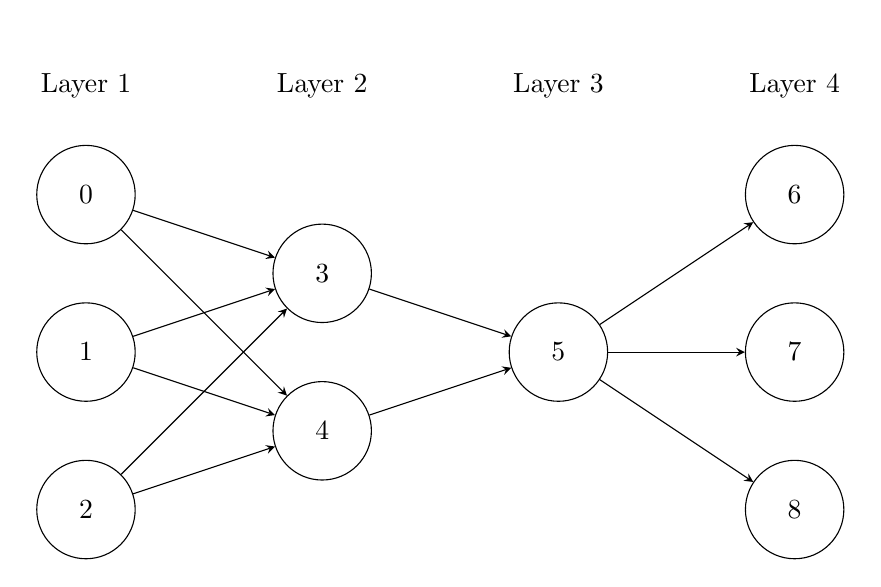
\begin{tikzpicture}[
			node distance=2cm and 3cm,
			every node/.style={draw, circle, minimum size=1.25cm},
			>=stealth,
		]
		% Layer 1 nodes
		\node[] (A1) at (0,2) {$0$};
		\node[] (A2) at (0,0) {$1$};
		\node[] (A3) at (0,-2) {$2$};

		% Layer 2 nodes
		\node[] (B1) at (3,1) {$3$};
		\node[] (B2) at (3,-1) {$4$};

		% Layer 3 node
		\node[] (C1) at (6,0) {$5$};

		% Layer 4 nodes
		\node[] (D1) at (9,2) {$6$};
		\node[] (D2) at (9,0) {$7$};
		\node[] (D3) at (9,-2) {$8$};

		% Connections from Layer 1 to Layer 2
		\draw[->] (A1) -- (B1);
		\draw[->] (A1) -- (B2);
		\draw[->] (A2) -- (B1);
		\draw[->] (A2) -- (B2);
		\draw[->] (A3) -- (B1);
		\draw[->] (A3) -- (B2);

		% Connections from Layer 2 to Layer 3
		\draw[->] (B1) -- (C1);
		\draw[->] (B2) -- (C1);

		% Connections from Layer 3 to Layer 4
		\draw[->] (C1) -- (D1);
		\draw[->] (C1) -- (D2);
		\draw[->] (C1) -- (D3);

		% Labels for the layers
		\node[draw=none, above=0cm of A1] {Layer 1};
		\node[draw=none, above=1cm of B1] {Layer 2};
		\node[draw=none, above=2cm of C1] {Layer 3};
		\node[draw=none, above=0cm of D1] {Layer 4};
	\end{tikzpicture}
	\caption{P2P-LLM Network Directed Graph}
	\label{fig:layered_graph}
\end{figure}

Due to this property, the P2P network graph is a directed acyclic graph (DAG). This means that there are efficient
algorithms to find the shortest path between two nodes. The first step is to perform a topological sort on the nodes in the network.
This is an ordering of the nodes such that all neighbors of a node come after the node in the ordering.
For any graph $G = (V, E)$ a topological ordering is an order $\prec$ on $V$ such that if $(u \rightarrow v) \in E$ then $u \prec v$.
For example, a topological ordering of the DAG in Figure \ref{fig:layered_graph} is $[0,1,2,3,4,5,6,7,8]$.
The algorithm for topological sort is shown in Appendix \ref{app:topo_sort}. With the topological order, dynamic programming can be used to find the shortest path in the network.
This algorithm will iterate over the ordering, and search all the node's neighbors for the one with the lowest weight.
The full algorithm is shown in Appendix \ref{app:shortest_path}. Most importantly, both the topological sort and path finding algorithm run in linear time
with a computational complexity of $O(|V| + |E|)$.

\subsection{Pareto Efficiency}

The optimal path is well defined when weights for nodes are clearly defined, but there is not an apparent way to define
weights for nodes in this case. In the P2P-LLM network, there are two competing criterion that define the weight of node: computational cost and price.
The algorithm described above uses a single objective (SO), while the optimal path in the network is a multi-objective (MO) optimization problem.
There are several way to find optimal solutions to MO optimization problems \citep{1599245}. The simplest way is to convert it to a SO optimization problem, and
since the shortest path algorithm is designed for SO objective, it is the most practical solution for this task. In order to reframe the problem as a single objective,
a weighed aggregate of the objectives is used. In the case for the peer-to-peer network, the SO is a weighed sum of computational cost $c_i$ and price $p_i$.
The objective, or weight, of a node, $w_i$ is defined as.

\begin{equation}
	w_i = \alpha \cdot p_i + (1 - \alpha) \cdot c_i
	\label{eq:weight}
\end{equation}

\begin{figure}
	\centering
	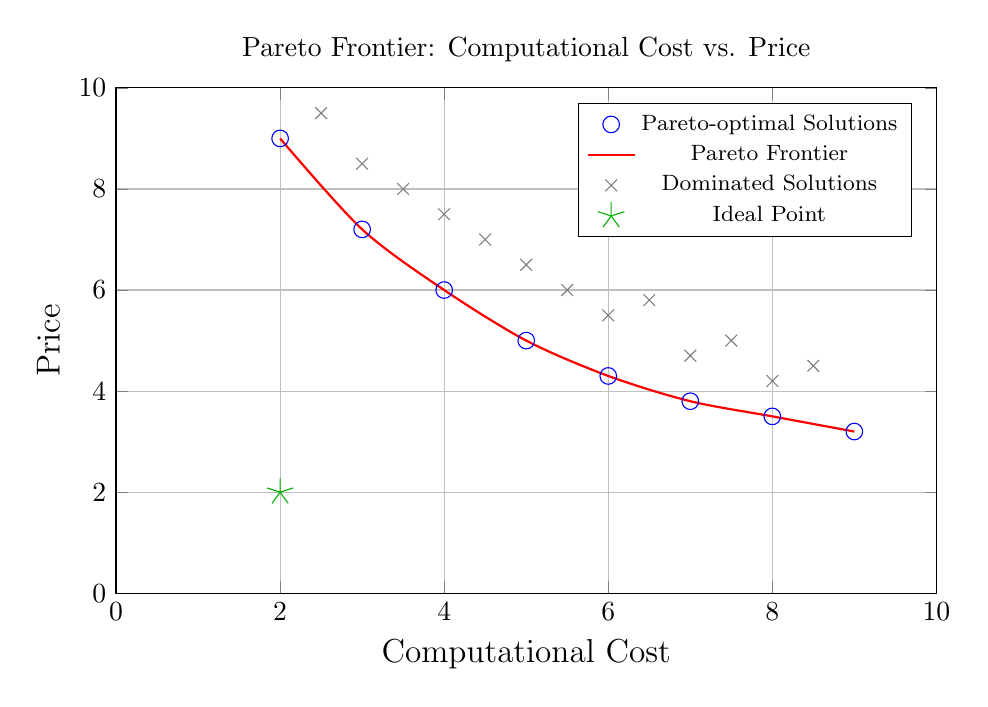
\begin{tikzpicture}
		\begin{axis}[
				width=12cm,
				height=8cm,
				xlabel={Computational Cost},
				ylabel={Price},
				xlabel style={font=\large},
				ylabel style={font=\large},
				xmin=0, xmax=10,
				ymin=0, ymax=10,
				xtick={0,2,4,6,8,10},
				ytick={0,2,4,6,8,10},
				grid=both,
				title={Pareto Frontier: Computational Cost vs. Price},
				legend pos=north east,
				legend style={font=\footnotesize}
			]

			% Scatter plot of solutions
			\addplot[only marks, mark=o, mark size=3pt, blue] coordinates {
					(2,9) (3,7.2) (4,6) (5,5) (6,4.3) (7,3.8) (8,3.5) (9,3.2)
				};

			% Pareto frontier
			\addplot[thick, red, smooth] coordinates {
					(2,9) (3,7.2) (4,6) (5,5) (6,4.3) (7,3.8) (8,3.5) (9,3.2)
				};

			% Sample dominated solutions
			\addplot[only marks, mark=x, mark size=3pt, gray] coordinates {
					(2.5,9.5) (3.5,8) (4.5,7) (5.5,6) (6.5,5.8) (7.5,5) (8.5,4.5)
					(3,8.5) (4,7.5) (5,6.5) (6,5.5) (7,4.7) (8,4.2)
				};

			% Ideal point (non-achievable)
			\addplot[only marks, mark=star, mark size=5pt, green!70!black] coordinates {
					(2,2)
				};

			% Add legend
			\legend{Pareto-optimal Solutions, Pareto Frontier, Dominated Solutions, Ideal Point};

		\end{axis}
	\end{tikzpicture}
	\caption{Pareto Frontier}
	\label{fig:Pareto-optimal}
\end{figure}

However, this assumes that the parameter $\alpha$ is known a priori. In general, there are many equivalent optimal solutions in a MO optimization problem.
These are known and Pareto-optimal solutions. They are solutions such that there is no way to improve one objective without degrading any other objectives.
A solution is said to be Pareto-optimal if there are no other solutions that dominate it. A solution $x_1$ dominates $x_2$ if
\begin{enumerate}
	\item $\forall i, f_i(x_1) \leq f_i(x_2)$ and
	\item $\exists i, f_i(x_1) < f_i(x_2)$
\end{enumerate}
where $f_i()$ is the utility for the $i$th objective.

The set of all Pareto-optimal solutions forms a frontier (Figure \ref{fig:Pareto-optimal}) of equivalent solutions, but there is not a clear choice on which one should be used.
In the case of the SO weighted aggregate used in the P2P-LLM network, the parameter $\alpha$ decides where on the Pareto frontier the optimal solution lies.
Due to this, each node can independently decide the importance of price and computational cost in the optimal path through the network by choosing the parameter $\alpha$.

\subsection{Revenue Optimization}

Each peer additionally has to choose a price to charge for other peers to use their computation.
Logically, each node will act in its self-interest and choose the price that maximizes revenue.
If the price is too high, peers will choose equivalent nodes serving the same layers,
while if the price is too low, the total revenue will be less than ideal.
The price they choose should reflect the current state of the network, and adapt to changing conditions.
In this context, price optimization become difficult as it is a dynamic environment
and a uniform pricing rule would not result in optimal revenue.
In the P2P-LLM network, a peer only has to compete with other peers serving the same layers.
This can be exploited to narrow down the complexities of this problem.
Working with this leads to the conclusion that a node's price should be determined
by its own price and computational cost and the price and computational cost of all other peers serving the same layers.

\begin{figure}
	\centering
	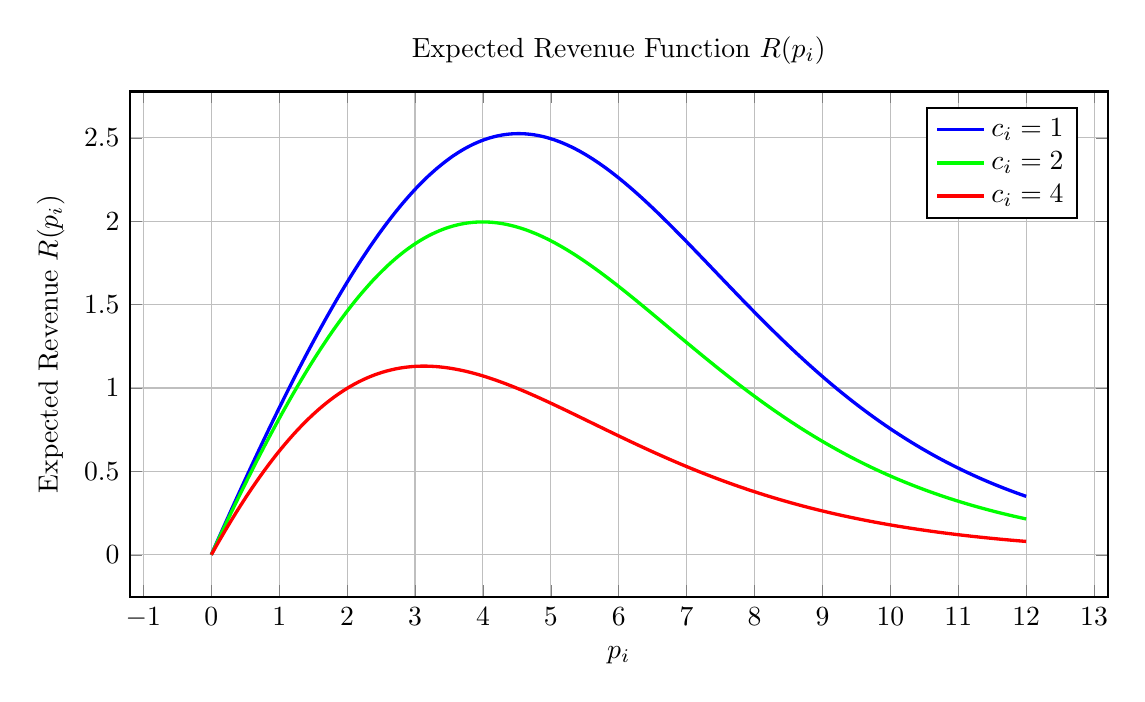
\begin{tikzpicture}
		\begin{axis}[
				width=14cm,
				height=8cm,
				xlabel={$p_i$},
				ylabel={Expected Revenue $R(p_i)$},
				domain=0:12,
				samples=200,
				legend pos=north east,
				grid=major,
				thick,
				every axis plot/.append style={very thick},
				title={Expected Revenue Function $R(p_i)$}
			]

			% Constant denominator
			\def\C{0.05}

			% Plot the function for different constants in numerator
			\addplot[color=blue] {(x)*(exp(-(0.5*x+0.5))/(exp(-(0.5*x+0.5)) +\C))};
			\addlegendentry{$c_i = 1$}
			\addplot[color=green] {(x)*(exp(-(0.5*x+1))/(exp(-(0.5*x+1)) +\C))};
			\addlegendentry{$c_i = 2$}
			\addplot[color=red] {(x)*(exp(-(0.5*x+2))/(exp(-(0.5*x+2)) +\C))};
			\addlegendentry{$c_i = 4$}

		\end{axis}
	\end{tikzpicture}
	\caption{Effect of Computational Cost on Expected Revenue}
	\label{fig:exp_rev}
\end{figure}

If we can define a revenue function based on these parameters, then the optimal price can be found by maximizing this function with respect to $p_i$.
The revenue a node receives for a single peer using the network would be its price multiplied by the probability of being chosen in the optimal path.

\begin{equation}
	R(p_i) = p_i \cdot \mathbb{P}(w_i)
	\label{eq:revenue}
\end{equation}

The probability that a node is chosen is related to its weight (Equation \ref{eq:weight}).
In order to get a distribution across all weights in the node's layer, the Boltzmann distribution \citep{boltzmann1868studien} can be used.
This distribution give the probability that a system will be in certain state.

\begin{equation}
	\mathbb{P}(\epsilon_i) = \frac{e^{- \epsilon_i / kT}}{\sum_{j=1}^{M}e^{- \epsilon_j / kT}}
	\label{eq:Boltzmann}
\end{equation}

where $\epsilon_i$ is the energy for state $i$, $k$ is the Boltzmann constant, and $T$ is the temperature of the system.
For the purposes of the P2P-LLM network, $k$ and $T$ are dropped and $\epsilon_i$ is $w_i$ (Equation \ref{eq:weight}).
Using this method gives a smooth expected revenue function, and prices will reflect how much each nodes contributes to the network.
Specifically, if a nodes contributes more compute power to the network, demonstrated as a lower computational cost $c_i$, the optimal
price they will charge will be higher, and they will be rewarded with a higher expected revenue.
A visualization of how $c_i$ effects the expected revenue curve is shown in Figure \ref{fig:exp_rev}.

Now with the expected revenue function, the optimal price can be found by finding the price that maximizes $R(p_i)$.
Unfortunately, there is not a closed form solution to this problem, but there are methods that can be used.
Iterative pricing mechanism \citep{ecf80b8b-07bb-374f-ab3f-2cc6a349f689} are used to find optimal prices by making iterative changes to the price until it converges at an optimal point.
These methods work well for dynamic environment where the state of the market is continuously changing.
For example, gradient ascent has been used for forex investing with algorithmic trading \citep{su142215328}.
The gradient ascent algorithm is very similar to the gradient descent algorithm \citep{cauchy1847methode} commonly used in machine learning.
The key difference is that it seeks to maximize a function's value rather minimize it.
Gradient ascent can be applied in the P2P-LLM network to maximize the expected revenue function, $R(p_i)$, with respect to price.
It is defined as

\begin{equation}
	\mathbf{x}_{t+1} = \mathbf{x}_t + \eta \nabla f(\mathbf{x}_t)
	\label{eq:grad}
\end{equation}

where $\mathbf{x}_t$ is the parameter vector at iteration $t$
,$\mathbf{x}_{t+1}$ is the updated parameter vector,
$\eta$ is the learning rate (step size)
, and $\nabla f(\mathbf{x}_t)$ is the gradient of the objective function $f$ at point $\mathbf{x}_t$.

Applying this to the revenue function, $R(p_i)$, we can get an update rule for the price.
The gradient of $R$ with respect to $p$ is
$$\diffp{R}{p} = \mathbb{P}(w)(1 + \alpha p \cdot (\mathbb{P}(w) - 1))$$

Using this with the gradient ascent algorithm (Equation \ref{eq:grad}), the price update rule is

\begin{equation}
	p_{t+1} = p_t + \eta \diffp{R}{{p_t}}
	\label{eq:optim_price}
\end{equation}

As all nodes continually update their prices, they will converge on the price that gives
maximum revenue for each node individually. Once this happens the network will be in a steady state where
no node will want to change its price.

\subsection{Network Equilibrium}

When all nodes are at the state of equilibrium, each layer in the network is at a Nash-Equilibrium (NE), meaning that any deviation in price
will result in a lower expected revenue. Formally this is defined as the utility of the optimal strategy being greater than or equal to any single deviation.
In the P2P-LLM network, the utility is just the revenue function $R$.
A price profile $p^*$ for a layer is a NE when

\begin{equation}
	u_i(p_i^*, p^*_{-i}) \geq u_i(p_i, p^*_{-i}) \forall p_i \in \mathbb{R}
\end{equation}

This is a equilibrium for an individual layer in the network, but the whole network may
not be at equilibrium. If the peers in the network are not evenly distributed,
some layers may have less peers serving them, which will lead to inefficiencies.
Ideally the computational power in the network will be evenly split between all layers
in the LLM. In an unbalanced state, this will lead to some nodes benefiting by changing which layers of the LLM they serve.

The optimal layer for a given node is the one in which they will have the largest
share of computation. The percentage of computation a node has can be found by normalizing the
computational cost across a layer. A reciprocal norm is used to find the share of computational power in the layer.
It is defined as

\begin{equation}
	s_l(c_i) = \frac{c_i^{-1}}{\sum_{j=i}^{n_l}c_j^{-1}}
	\label{eq:norm}
\end{equation}

where $l$ is the layer, $n_l$ is the number of nodes serving the layer $l$, and $c_i$ is the computational cost.
The optimal layer for a node, is the one that maximizes this value.

\begin{equation}
	l^* = \text{max}_l \quad s_l(c_i)
	\label{eq:max}
\end{equation}

In the P2P-LLM network, peers will periodically change layers if they are not already in the optimal state.
Changing layers will increase the peers expected revenue while also increasing the throughput of the network overall.
In this case the incentives of the individual nodes are aligned with the whole network overall.
When no peers have a useful change then the network is in an efficient state.

\section{Cryptoeconomics}
The P2P-LLM network requires a secure, transparent, and decentralized mechanism to facilitate transactions between peers.
The blockchain provides a secure and decentralized way to allow peers to form contracts with eachother
and exchange payment in cryto-currencies for computation.
Cryptoeconomics has proven to be successful in the past with some application being in
resources trading through the blockchain. Specifically, research has been done to enable peer-to-peer surplus energy on the blockchain \citep{WONGTHONGTHAM2021107299}.
For the P2P-LLM network, the blockchain serves three primary functions: (1) recording the state of the network including available nodes and their capabilities, (2) facilitating secure payments between peers, and (3) executing smart contracts that govern computational resource sharing.

\subsection{Blockchain}

Blockchain technology provides an ideal foundation for this system, as it offers immutability, transparency, and security without relying on a central authority.

The blockchain implementation for P2P-LLM employs a Proof-of-Stake (PoS) consensus mechanism rather than the energy-intensive Proof-of-Work (PoW) used in systems like Bitcoin \citep{nakamoto2008bitcoin}. This design choice aligns with the goal of resource efficiency, as PoS validators are selected based on the quantity of tokens they have staked, consuming significantly less energy than PoW mining operations \citep{saleh2021blockchain}. This approach is particularly appropriate for a system focused on computational resource optimization.

Each block in the P2P-LLM blockchain contains transactions representing computational resource exchanges between peers. These transactions include metadata such as the identity of the participating nodes, the layers being computed, the computational cost, and the agreed-upon price. Additionally, the blockchain maintains a distributed registry of all active nodes and their capabilities ($\ell_i$, $c_i$, $p_i$), which is critical for the path-finding algorithm described in Section 3.1.

To ensure scalability, the P2P-LLM blockchain implements a sharding mechanism that partitions the network state by model layers. This design allows transactions related to specific model layers to be processed in parallel, significantly increasing throughput as the network grows. Each shard maintains its own state and processes transactions independently, with periodic cross-shard communication to maintain overall network consistency \citep{yu2020survey}.

\subsection{Contracts}

Smart contracts form the backbone of the interaction mechanism in the P2P-LLM network. These self-executing contracts with the terms of agreement directly written into code automate the negotiation, execution, and settlement processes between peers without requiring trust or intermediaries.

In the P2P-LLM network, three types of smart contracts are employed:

\begin{enumerate}
	\item \textbf{Registration Contracts}: These contracts handle the onboarding of new nodes to the network. When a node joins, it executes a registration contract that records its capabilities ($\ell_i$, $c_i$, $p_i$) on the blockchain. This contract also requires the node to stake a minimum amount of tokens as collateral, which can be forfeited if the node behaves maliciously or fails to deliver promised computational resources.
	\item \textbf{Service Level Agreements (SLAs)}: These contracts formalize the terms of computational resource sharing between peers. An SLA contract specifies the model layers to be computed, the expected computational performance (in terms of latency and throughput), the price per computation, and penalties for non-compliance. The contract is automatically executed when a peer requests computation, with payment held in escrow until the computation is successfully completed and verified.
	\item \textbf{Payment Channels}: To minimize transaction costs and latency, the P2P-LLM network implements payment channels similar to Bitcoin's Lightning Network \citep{poon2016bitcoin}. These channels allow peers to conduct multiple transactions off-chain, only settling the final balance on the blockchain when the channel is closed. This approach is particularly valuable for high-frequency, low-value transactions that are common in LLM inference operations.
\end{enumerate}

The execution of these contracts is governed by a verification mechanism that ensures computational integrity. When a node performs computation for another peer, the input, output, and intermediate states are cryptographically hashed and recorded on the blockchain. This creates a verifiable proof of computation that can be used to resolve disputes and ensure that nodes are correctly performing their assigned tasks.

To optimize contract execution in the dynamic environment of the P2P-LLM network, an adaptive pricing mechanism based on the concepts described in Section 3.3 is used. This mechanism allows for continuous adjustment of prices based on network conditions, ensuring that nodes are appropriately incentivized to provide computational resources where they are most needed.

The combination of these contract mechanisms creates a self-regulating marketplace for computational resources that aligns individual incentives with the overall efficiency of the network. Nodes are rewarded for providing reliable, cost-effective computation, while clients can access LLM capabilities at competitive prices without relying on centralized service providers.

\section{Experiment Setup}

To evaluate the performance, stability, and efficiency of the propose P2P-LLM protocol, I implemented a simulated environment
to model the dynamics of the network.
The simulation explores the relationship between computational resource allocation, price optimization, and network equilibrium under various conditions without requiring the deployment of an actual LLM across distributed hardware.

\subsection{Simulation Framework}
The simulation framework implements a discrete event-based model of the P2P-LLM network, where each event corresponds to a peer action such as joining the network, processing requests, updating prices, or switching layers. The simulation progresses in timesteps, with each timestep representing a fixed duration (e.g., 1 second in simulated time). At each timestep, the following operations are performed:
\begin{enumerate}
	\item Process pending inference requests through the network
	\item Update node prices according to the gradient ascent algorithm (Equation \ref{eq:optim_price})
	\item Periodically, reallocate nodes to new layers (Equation \ref{eq:max})
	\item Create new contracts for peers without a pending contract
	\item Record metrics for analysis
\end{enumerate}
The simulation parameters can be configured to model various network sizes, LLM architectures, and peer behaviors, allowing for comprehensive sensitivity analysis.

\subsection{Network Configuration}

For the simulation, I chose to create a small network, with $n = 28$ total nodes, and a simulated LLM with $m = 4$ layers.
The parameters of the nodes in the network were randomly initialized
where $c_i \in (1,50)$, $l_i \in (1,20)$. All prices are intitially set at $1$. The inital state of the network not optimal with the peers being distributed between the $4$ layers in the configuration $[10, 4, 10, 4]$.
For simplicity, all nodes have an $\alpha$ value of $0.5$ and the $\eta$ used in the iterative pricing function is $1$.

\section{Results}

\begin{table}[t]
	\centering
	\caption{P2P-LLM Network Metrics at Different Iteration Steps (Model with 4 Layers, 200 Peers)}
	\label{tab:network-metrics}
	\begin{tabular}{ccccccc}
		\toprule
		\textbf{Iteration} & \textbf{Metric} & \textbf{Layer 1} & \textbf{Layer 2} & \textbf{Layer 3} & \textbf{Layer 4} \\
		\midrule
		\multirow{3}{*}{0}
		                   & Nodes           & 78               & 52               & 34               & 36               \\
		                   & Avg. Price      & 5.42             & 5.28             & 5.87             & 5.31             \\
		\midrule
		\multirow{3}{*}{100}
		                   & Nodes           & 62               & 48               & 43               & 47               \\
		                   & Avg. Price      & 5.89             & 5.96             & 5.72             & 5.68             \\
		\midrule
		\multirow{3}{*}{500}
		                   & Nodes           & 53               & 49               & 50               & 48               \\
		                   & Avg. Price      & 6.12             & 6.08             & 6.10             & 6.05             \\
		\midrule
		\multirow{3}{*}{1000}
		                   & Nodes           & 50               & 50               & 50               & 50               \\
		                   & Avg. Price      & 6.14             & 6.15             & 6.13             & 6.15             \\
		\midrule
		\multirow{3}{*}{5000}
		                   & Nodes           & 50               & 50               & 50               & 50               \\
		                   & Avg. Price      & 6.13             & 6.14             & 6.14             & 6.13             \\
		\bottomrule
	\end{tabular}
\end{table}

% Manual newpage inserted to improve layout of sample file - not
% needed in general before appendices/bibliography.
%
\newpage

\appendix
\section{Topological Sort}
\label{app:topo_sort}
\begin{algorithm}
	\caption{Topological Sort of a Directed Acyclic Graph (DAG)}
	\begin{algorithmic}[1]
		\Require{A directed acyclic graph $G = (V, E)$}
		\Ensure{A linear ordering of vertices such that for every directed edge $(u, v)$, vertex $u$ comes before vertex $v$}

		\State $\text{result}[]$ \Comment An empty list to store the sorted vertices
		\State $\text{visited}[v] \rightarrow $false for all $v \in V$ \Comment A map to track visited vertices
		\State $\text{temp}[v] \rightarrow $ false for all$ v \in V$ \Comment A map to track vertices in the current recursion stack

		\For{each vertex $v \in V$}
		\If{$\text{visited}[v] = \text{false}$}
		\State DFS-Visit($G$, $v$, $\text{visited}$, $\text{temp}$, $\text{result}$)
		\EndIf
		\EndFor

		\State \Return Reverse($\text{result}$)

		\Function{DFS-Visit}{$G$, $u$, $\text{visited}$, $\text{temp}$, $\text{result}$}
		\State $\text{temp}[u] \gets \text{true}$ \Comment{Mark current vertex as being processed}

		\For{each vertex $v$ such that $(u, v) \in E$}
		\State DFS-Visit($G$, $v$, $\text{visited}$, $\text{temp}$, $\text{result}$)
		\EndFor

		\State $\text{temp}[u] \gets \text{false}$ \Comment{Mark $u$ as processed}
		\State $\text{visited}[u] \gets \text{true}$ \Comment{Mark $u$ as visited}
		\State Append $u$ to $\text{result}$
		\EndFunction
	\end{algorithmic}
\end{algorithm}

\newpage

\section{Shortest Path}
\label{app:shortest_path}
\begin{algorithm}
	\caption{Shortest Path in a DAG}
	\begin{algorithmic}[1]
		\Require{Graph $G = (V, E)$ with edge weights $w$, source vertex $s$, target vertex $t$, topological ordering $topo[]$ of $G$}
		\Ensure{Length of shortest path from $s$ to $t$ and the path itself}

		\State Initialize $dist[v] \gets \infty$ for all $v \in V$
		\State Initialize $prev[v] \gets \text{nil}$ for all $v \in V$
		\State $dist[s] \gets 0$

		\For{each vertex $u$ in topological order $topo[]$}
		\For{each outgoing edge $(u, v) \in E$}
		\If{$dist[v] > dist[u] + w(u, v)$}
		\State $dist[v] \gets dist[u] + w(u, v)$
		\State $prev[v] \gets u$
		\EndIf
		\EndFor
		\EndFor

		\State $path \gets \emptyset$ \Comment{Reconstruct the shortest path}
		\State $curr \gets t$
		\While{$curr \neq \text{nil}$}
		\State Prepend $curr$ to $path$
		\State $curr \gets prev[curr]$
		\EndWhile

		\State \Return $dist[t]$, $path$
	\end{algorithmic}
\end{algorithm}

\vskip 0.2in
\bibliography{main}

\end{document}
